\documentclass{IEEEtran}
\usepackage{bm}
\usepackage{amsmath}
\usepackage{amssymb}
\usepackage{booktabs}
\usepackage{algorithm}
\usepackage{algorithmicx}
\usepackage{algpseudocode}
\usepackage{stfloats}
\usepackage{graphicx}
\DeclareMathOperator*{\argmax}{arg\,max}
\DeclareMathOperator*{\argmin}{arg\,min}
\DeclareMathOperator*{\sigmoid}{sigmoid}

\renewcommand{\IEEEQED}{\IEEEQEDclosed}
\title{Optimal Fishing Strategy Based on Scientific Outlook on Development}
\author{
    Weitong~ZHANG, Yiwen~LU, Zifeng~KANG
    \thanks{Weitong~ZHANG 2015011493  \texttt{WeightZero@outlook.com}}
    \thanks{Yiwen~LU 2015011443  \texttt{ylu.thu15@gmail.com}}
    \thanks{Zifeng~KANG 2015011496  \texttt{kangzf15@mails.tsinghua.edu.cn}}
}
\begin{document}
\maketitle

\begin{abstract}
    The SOD incorporates scientific socialism, sustainable development, social welfare, a humanistic society, increased democracy, and, ultimately, the creation of a Socialist Harmonious Society. According to official statements by the CPC, the concept integrates ``Marxism with the reality of contemporary China and with the underlying features of our times, and it fully embodies the Marxist worldview on and methodology for development."
\end{abstract}

\section{Introduction}

With the rapid growth of modern society and technology, the depletion of resources has brought about jarring problems to environmentalists, economists and policy makers, and even serious threats to the survival of human beings. Even today, in most countries, how to rationally develop and use resources still remains a vital issue that requires collaboration of country leaders with ordinary people.

Fortunately, faced with this tough situation, leaders of Communist Party of China have proposed Scientific Concept of Development (SOD). The basic requirements of SOD are comprehensive, coordinated, and sustainable. In the light of SOD, development of our country aims to ensure profitability while maintain sustainability.

Thoughts of SOD are so inclusive and universal that we decide to apply them to fishery problems. As a renewable kind of resource, fish die and spawn hatch at a speed that we are able to calculate and predict, so it is feasible that we obtain satisfying strategy using these data. Furthermore, in order to provide practical advice to fishermen, previous studies have found that fixed-effort-harvest strategy may not only perform excellently in models or simulations, but have potential practical value as well. Yet among all such strategies, the gross yield can be extremely different, so there is still much work to do. 

According to principles of SOD, we develop two state-of-the-art models in this paper and obtain optimal fixed-effort-harvest strategy that not only satisfies harsh requirements on the fishery contract but also makes a great deal of profit for the company. We further believe this strategy is also applicable in real life. 

\section{Basic Assumptions}
\subsection{Features of Fish}
\begin{itemize}
\item {The maturing time period of involved fish is exactly 4 years, which means when the next year arrives, alive spawns of the first year hatch into 1-aged fish and alive $i$-aged fish grow into $(i+1)$-aged fish($i=1,2,3$), while alive 4-aged fish remain 4-aged.}
\item {Fish that share the same age are homogeneous, including weight, size, growth and spawning behavior and possibility to be harvested.}
\item {The amount of each fish group is continuously differentiable as a function of time.}
\item {All fish die at all times at a constant speed, with a total annual natural fatal rate of 0.8 .}
\item {All fish spawn instantaneously, and all spawns are homogeneous. }
\end{itemize}

\subsection{Features of Human Harvest}
\begin{itemize}
\item {Human harvest fish at all times at a speed proportional to fish amount at that time. The proportion coefficient is called \textit{fishing intensity}.}
\item {At the end of each year, if remaining fish of each group are not less than 80\% of saturation level, then in that year `fish productivity is not badly damaged'.}
\end{itemize}

\subsection{Notations}
We will use the notations in Tab. \ref{notations} in the following modeling and optimizing.

\begin{table}[h]
    \centering
    \caption{Notation table}
    \label{notations}
    \begin{tabular}{cc}
        \toprule
        Notation & Meaning \\ \midrule
        $x$ & The number of a certain group of fish \\
        $x_i$ & The number of $i$-aged fish \\
        $\bm X, \bm x$ & The number of all 4 groups of fish, 4-d vector\\
        $k$ & Fishing intensity of the 4-aged fish \\
        $t$ & Time, starting from 0 with the unit of year \\
        $\lambda$ & Rate of survival of fish, constant \\
        $y$ & The number of egg\\
        $y_i$ & The number of egg spawned by a certain fish $i$\\ 
        $\pmb C$ & Fishing intensity parameters matrix, constant, $4 \times 4$ matrix\\
        $\pmb D$ & Spawing parameters matrix, constant, $1 \times 4$ matrix\\
        $\mu$ & Rate of spawing, constant \\
        $\pmb T$ & Transform matrix of fish update, constant, $4 \times 4$ matrix\\
        $\bm x'$ & The number of fish in the next year, 4-d vector\\
        $\bm x_0, \bm X_0$ & The number of fish in the beginning of the year, 4-d vector\\
        $\mathrm I$ & $4 \times 4$ identity matrix\\
        $z$ & harvest in the next year\\
        $Z$ & total harvest\\
        $\Gamma$ & Penalty factor\\
        $\bm X_s$ & The number of fish in saturation state\\
        $\bm x_{sat,i}$ & The number of $i$-aged fish in saturation state\\
        $\bm K$ & The intensity for 5 years, 5-d vector\\
        \bottomrule
    \end{tabular}
\end{table}

\section{Model on Sustainable Harvesting} \label{model1}
Owing to the annual death ratio is 0.8, we assume that the number of fish $x$ obeys the distribution eq. \ref{eq1}

\begin{equation}
    \label{eq1}
    x = x_0 \exp(-\lambda t)
\end{equation}

while the unit of $t$ is year, we get $\lambda = \ln 5, \frac{\mathrm dx}{\mathrm dt} = -\lambda x$

Setting the fishing intensity of 4-aged fish to be $k$, we can get the one of 3-aged fish is $0.42k$, while the number of the four group of fish could be described as a 4-d vector $\bm x$ .

\subsection{Model on the first eight months}

We can use the differential equation eq. \ref{eq2} to describe the trend of the number of fish in each group

\begin{align}
    \label{eq2}
    -\frac{\mathrm d \bm x}{\mathrm d t} &= k \pmb C \bm x + \lambda \bm x \\
    \pmb C &= \begin{pmatrix}0&0&0&0\\0&0&0&0\\0&0&0.42&0\\0&0&0&1\end{pmatrix}
\end{align}
\subsection{Model on the last four months}
Set the number of eggs is $y$, and for each fish, we set the rate of spawning as $\mu$, i.e. $\frac {\mathrm d y_i}{\mathrm d t} = \mu$, where $y_i$ is the eggs spawned by a certain fish $i$. Then we get the following differential equation eq. \ref{eq3}

\begin{align}
    \label{eq3}
    \frac {\mathrm d y}{\mathrm d t} &= \mu \pmb D \bm x\\
    -\frac{\mathrm d \bm x}{\mathrm d t} &=\lambda \bm x\\
    \pmb D &= \begin{pmatrix} 0 & 0 & 1.109\times10^5/2&1.109\times10^5\end{pmatrix}
\end{align}

From the average spawning rate, we can get that $\mu = 3$.

\subsection{Model on the changes of the next year}

After a year, some eggs spawned in the first year would be the 1-aged fish, according to the survival ratio. Therefore, we can get the following transform function eq. \ref{eq4}

\begin{align}
    \label{eq4}
    y &= 0\\
    \bm x &= \pmb T \bm x +\begin{pmatrix} f(y)&0&0&0\end{pmatrix}^{\mathrm T}\\
    f(y) &= \frac{1.22\times 10 ^{11}y}{1.22\times 10 ^{11} + y}\\
    \pmb T &= \begin{pmatrix} 0 & 0 & 0 & 0 \\ 1& 0 & 0 & 0 \\ 0 & 1 & 0 & 0 \\0 & 0 & 1 & 1 \end{pmatrix}
\end{align}

\subsection{Solve the function}

Now We can conclude all of the function above to solve the equation \ref{eq5} of $\bm x$: $\bm x' = \bm x$ based on $k$, where $\bm x'$ is the number of fish next year:  

\begin{align}
    \bm x' &= \bm x_0\\
    \label{eq5}
    \bm x' &= \pmb T \exp(-\frac{\pmb A_2 + 2 \pmb A_1}{3})\bm x_0 +\begin{pmatrix} f(\pmb B \exp(-\frac{2\pmb A_1}{3})\bm x_0)\\0\\0\\0\end{pmatrix}
\end{align}
\begin{align}
    \pmb A_1 &= k\pmb C + \lambda \pmb I\\
    \pmb A_2 &= \lambda \pmb I\\
    \pmb B &= (\mu \pmb D A_2^{-1}(\pmb I - \exp(-\pmb A_2/3)))
\end{align}

Therefore, we can get the relationship between $\bm x$ and $k$ numerically.
\subsection{Relation bewteen Harvest and Fishing Intensity}
The total of harvest $z$ could be described as the following function eq. \ref{eq6}
\begin{align}
    \label{eq6}
    \frac {\mathrm dz}{\mathrm dt} &= k\pmb C \bm x\\
    z &= k\pmb C\int_0^{2/3}\exp(-\pmb A_1t)\mathrm dt\bm x_0 \\ 
    &= k\pmb C  A_1^{-1} (1-\exp(-2\pmb A_1/3))\bm x_0
\end{align}
where $\bm x_0$ would be the initial number of fish.


%%%%%%%%%%%%%%%%%%%%%%%%%%%%%%%%%%%%%%%%%
%
%         RESULT FOR PART 1
%
%%%%%%%%%%%%%%%%%%%%%%%%%%%%%%%%%%%%%%%%%
\section{Model on five successive fishing}\label{model2}

According to the analysis above, we can also calculate the number of fish $\bm x'$ in the next year by eq.\ref{eq5}, and we can also get the sum of the harvest $z$, let's set the relationship between them as eq. \ref{eq7}

\begin{equation}
    \label{eq7}
    \bm x' = F(\bm x, k), \bm z = G(\bm x,k)
\end{equation}

Therefore, the total harvest and the number of fish remaining after 5 years could be calculate by the following algorithm \ref{A1}

\begin{algorithm}[h]
    \caption{Calculate the harvest and the number of fish}\label{A1}
    \begin{algorithmic}
        \Require Initial state $\bm X_0$, fishing strategy $\bm K = [k_1,\cdots,k_5]$ 
        \Ensure Sum of harvest $Z$ and the number of fish after 5 years $\bm X$
        \State Let $\bm X = \bm X_0, Z = 0$
        \For{$i$ in $[1,\cdots,5]$}
        \State $Z \leftarrow Z + G(\bm X,\bm K_i)$
        \State $\bm X \leftarrow F(\bm X, \bm K_i)$
        \EndFor
    \State \Return $Z$ and $\bm X$
    \end{algorithmic}
\end{algorithm}

According to the contract, the productive ability could not be bitterly destroyed after 5 years. However, this rule is a relatively blurry one, which needs a quantitative description. In the following discussing, we will try several method to decide the factor $\Gamma \le 1$, which is used to describe the loss of the productive ability. And our objective function would be $H(\bm K) = Z\Gamma$, while $Z$ is calculated by algorithm \ref{A1}. We are about to maximize $H(\bm K)$

\subsubsection{Baseline of productive ability}

First of all, we need to provide a baseline of productive ability. It is reasonable to guess that the maximum of the number of fish is the steady state with $k = 0$, according to the survival rate of the eggs, we can guess that the 1-aged fish is limited to the following value:

\begin{equation}
    x_1 = \lim_{y\to\infty} f(y) = 1.22 \times 10^{11}
\end{equation}

Using this value as the 1-aged fish, we can conclude that the saturation of the number of fish is obeying the following function:

\begin{equation}
    \begin{cases}
        x_2 = 0.2 x_1\\
        x_3 = 0.2^2 x_1\\
        x_4 = 1.25 \times 0.2^3 x_1
    \end{cases}
\end{equation}

Therefore, the saturation of the number of fish should be described as eq. \ref{eq8}

\begin{equation}
    \label{eq8}
    \bm X_s = 1.22 \times 10^{11}\begin{pmatrix}1 & 0.2 & 0.04 & 0.01\end{pmatrix}^\mathrm T
\end{equation}

\subsubsection{Penalty I. Comparison with the saturation number of fish}

It is obvious that it is a good idea to keep the number of the fish similar to the saturation one $\bm X_s$, therefore, we can design our object function as eq. \ref{eq9}
\begin{align}
    \label{eq9}
    \Gamma &= \sigmoid(\frac{(\Theta^\mathrm T)(\bm X / \bm X_s - 0.8)}{\sigma})
\end{align}
where $\sigma$ and $\Theta$ are designed manually, $\Theta$ is a $4 \times 1$ vector, and the division $\bm X / \bm X_s$ is the element-size devision. $\bm X$ and $Z$ could be calculate by symbolic computation in algorithm \ref{A1}

The sigmoid function should be described as eq. \ref{eq10}

\begin{equation}
    \label{eq10}
    \sigmoid(x) \triangleq \frac1{1 + \exp(-x)}
\end{equation}

We are about to maximize the $H(\bm K)$, and it is obvious that if the final number of fish $\bm X$ is much closer to $\bm X_s$, the $H(\bm K)$ would be also increasing.

\subsubsection{Optimizer: the Gradient Descent method}

By using computer algebra method, we can easily get the derivative of the object function, i.e. $\frac{\partial H}{\partial \bm K}$, and therefore we could use GD method to get the better fishing strategy.

%%%%%%%%%%%%%%%%%%%%%%%%%%%%%%%%%%%%%%%%%%%%%%%%%%%%%%%%%%%%%%%%%%
%
%              RESULT FOR G.D. METHOD
%
%%%%%%%%%%%%%%%%%%%%%%%%%%%%%%%%%%%%%%%%%%%%%%%%%%%%%%%%%%%%%%%%%%%

\subsubsection{Other Optimizer and Other Penalty Functions}

The penalty mentioned above is focus on the changing of the numbers, however, it is also possible that different combinations of numbers can gain the same productive ability. Therefore, the penalty here is more curious about the total harvest in the later years.

\begin{itemize}
    \item {Short Term Assess Method

    By running the body of the loop in algorithm \ref{A1}, we can calculate the harvest of the next year $Z'(k) = G(\bm X,k)$, let the penalty factor $\Gamma$ be eq. \ref{eq11}
    
    \begin{equation}
        \label{eq11}
        \Gamma \triangleq \min_{k \in[1,2,\cdots,20]} \frac{G(\bm X,k)}{G(\bm X_s,k)}
    \end{equation}
    }

    \item {Long Term Assess Method
        
    According to the further analysis, however, the short term assess method do not sound like a good idea, which is because the productive ability described by this method cannot take the 1-aged fish and 2-aged fish into consideration for it is only consider the next year, when the 1-aged one and 2-aged one are not abot to spawn. Hence, we need to expand the short-term method into a relatively long-term method. For the reason that the periodic time of the fish is about 4 years, we use the 4-year-term should be better. The $\Gamma$ function should be desctibed as eq. \ref{eq12}, in which we calculate the total harvest by algorithm \ref{A1} (or a relatively similar algorithm) and set the result with the initial state $\bm X$ and intensity (which is constant during the 4 years) $k$ as $R(\bm X,k)$
    
    \begin{equation}
        \label{eq12}
        \Gamma \triangleq \min_{k \in[1,2,\cdots,20]} \frac{R(\bm X,k)}{R(\bm X_s,k)}
    \end{equation}
    In which the total harvest could be calculated also by algorithm \ref{A1}.

    Further experiment shows that while it is inaccurate, it is also not a good idea to choose a much longer period, owing to the fact that the harvest in the last few years and the number of the fish then will arrive at a relatively stable state, which would cover the initial loss. In a few words, a 4-year-term is a good idea.
        }
\end{itemize}

For the two $\Gamma$ function based on harvest mentioned above, the optimization based on gradient might not sound like a good idea, therefore, we use MATLAB\textsuperscript\textregistered \ toolbox\textsuperscript{\cite{MATLABOptimizationToolbox}} to solve this problems. By using functions like fmincon (which is based on the calculated gradient), and GA (which completely treat the object function as a blackbox), the optimization process performs well and generate the result just like we want.

\section{Result}

\subsection{Solution to the first problem}\label{result1}

Applying the model described in Part \ref{model1}, under the constraint of sustainable harvesting, the annual harvest $z$ can be represented as a function w.r.t. the fishing intensity of 4-aged fish $k$. The analytical expression is derived with SymPy \textsuperscript{\cite{Joyner:2012:OSC:2110170.2110185}}. The function is numerically plotted in Figure \ref{plot1}. Note that $z$ is meaningful if and only if $z>0$, and thus the feasible region of $k$ is automatically determined.

\begin{figure}[h]
	\centering
	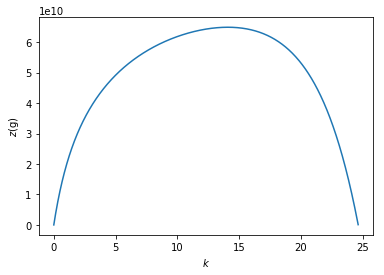
\includegraphics[width=\columnwidth]{plot1}
	\caption{The relationship between annual harvest $z$ and fishing intensity $k$\label{plot1}}
\end{figure}

The relationship between $z$ and $k$ is not monotonous, which agrees with our intuition: when $k$ is too small, the fishing intensity is too small to exploit the resources; when $k$ is too large, the number of fishes in the steady state is decreased, affecting the harvest. By performing a linear search on $k$, the optimal fishing strategy can be determined:

$$\begin{cases}\argmax\limits_k z(k) \approx 14.09\\\max\limits_k z(k) \approx 6.49\times 10^{10} \end{cases}$$

\subsection{Solution to the second problem using Gradient Descent}

Applying the model described in Part \ref{model2}, the optimization problem can be formulated as follows:

\begin{equation}\begin{aligned}
	\label{J}
	\min\limits_{ \boldsymbol{K}} J(\boldsymbol{K}) = -z( \boldsymbol{K}) - M \sum\limits_{i=1}^4 g(\frac{x_i}{x_{ \mathrm{sat}, i}})
\end{aligned}\end{equation}

In equation \ref{J}, $\boldsymbol{k}\in \mathbb{R}^5$ stands for the intensity in the five years, $M$ is a large coefficient for the penalty of over-fishing (chosen as $1.22\times 10^{11}$ in practice), and $g$ is a sigmoid function centered at 0.8:
$$g(\lambda) = \frac1{1+ \exp(-k(\lambda - \lambda_0))}$$
where $\lambda_0 = 0.8$ and $k$, representing the bandwidth of the sigmoid function, is experimentally determined as 100. A plot of $g$ is shown in Figure \ref{g}.

\begin{figure}[h]
	\centering
	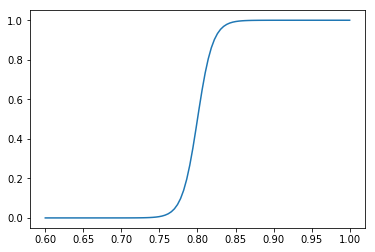
\includegraphics[width=0.6\columnwidth]{g}
	\caption{The smooth thresholding function used for penalty of over-fishing\label{g}}
\end{figure}

Since $J$ defined in equation \ref{J} is differentiable w.r.t. all elements of $\boldsymbol{K}$, it can be optimized using gradient descent: $\boldsymbol{K}$ is initialized to a random vector $\boldsymbol{K}_0$, and in each iteration:

$$\boldsymbol{K}\leftarrow \boldsymbol{K} - \alpha \frac{\partial J}{\partial \boldsymbol{K}}$$

The process is repeated until convergence. In practice, the gradients are symbolically derived with SymPy, $\boldsymbol{K}_0$ is drawn from normal distribution $\mathcal{N}(10, 2^2)$, and the coefficient $\alpha$ is experimentally determined as $3\times 10^{-10}$. Random initialization is repeated for 10 times, all of which converge to essentially the same solution except for negligible numerical errors:

\begin{equation}\label{K}\boldsymbol{K} = [18.59, 15.09, 17.77, 17.42, 17.56]\end{equation}
    
The identical convergence result gives us confidence that $\boldsymbol{K}$ in equation \ref{K} is a good approximation of the global optimal solution.

The result may be intuitively explained as follows: based on the observation that the initial values for number of fishes are above the saturation values, the intensity adopted in the first year can be larger than the ``normal'' values; the intensity is decreased in the second year to allow more fish to grow up; starting from the third year, a relatively steady state is reached, and therefore the intensity for the last three years remain stable. As a whole, the intensity values are larger than the result presented in Part \ref{result1}, since the requirement that ``the productive ability could not be bitterly destroyed'' is slacker than the requirement of sustainable development.

\begin{figure}[h]
    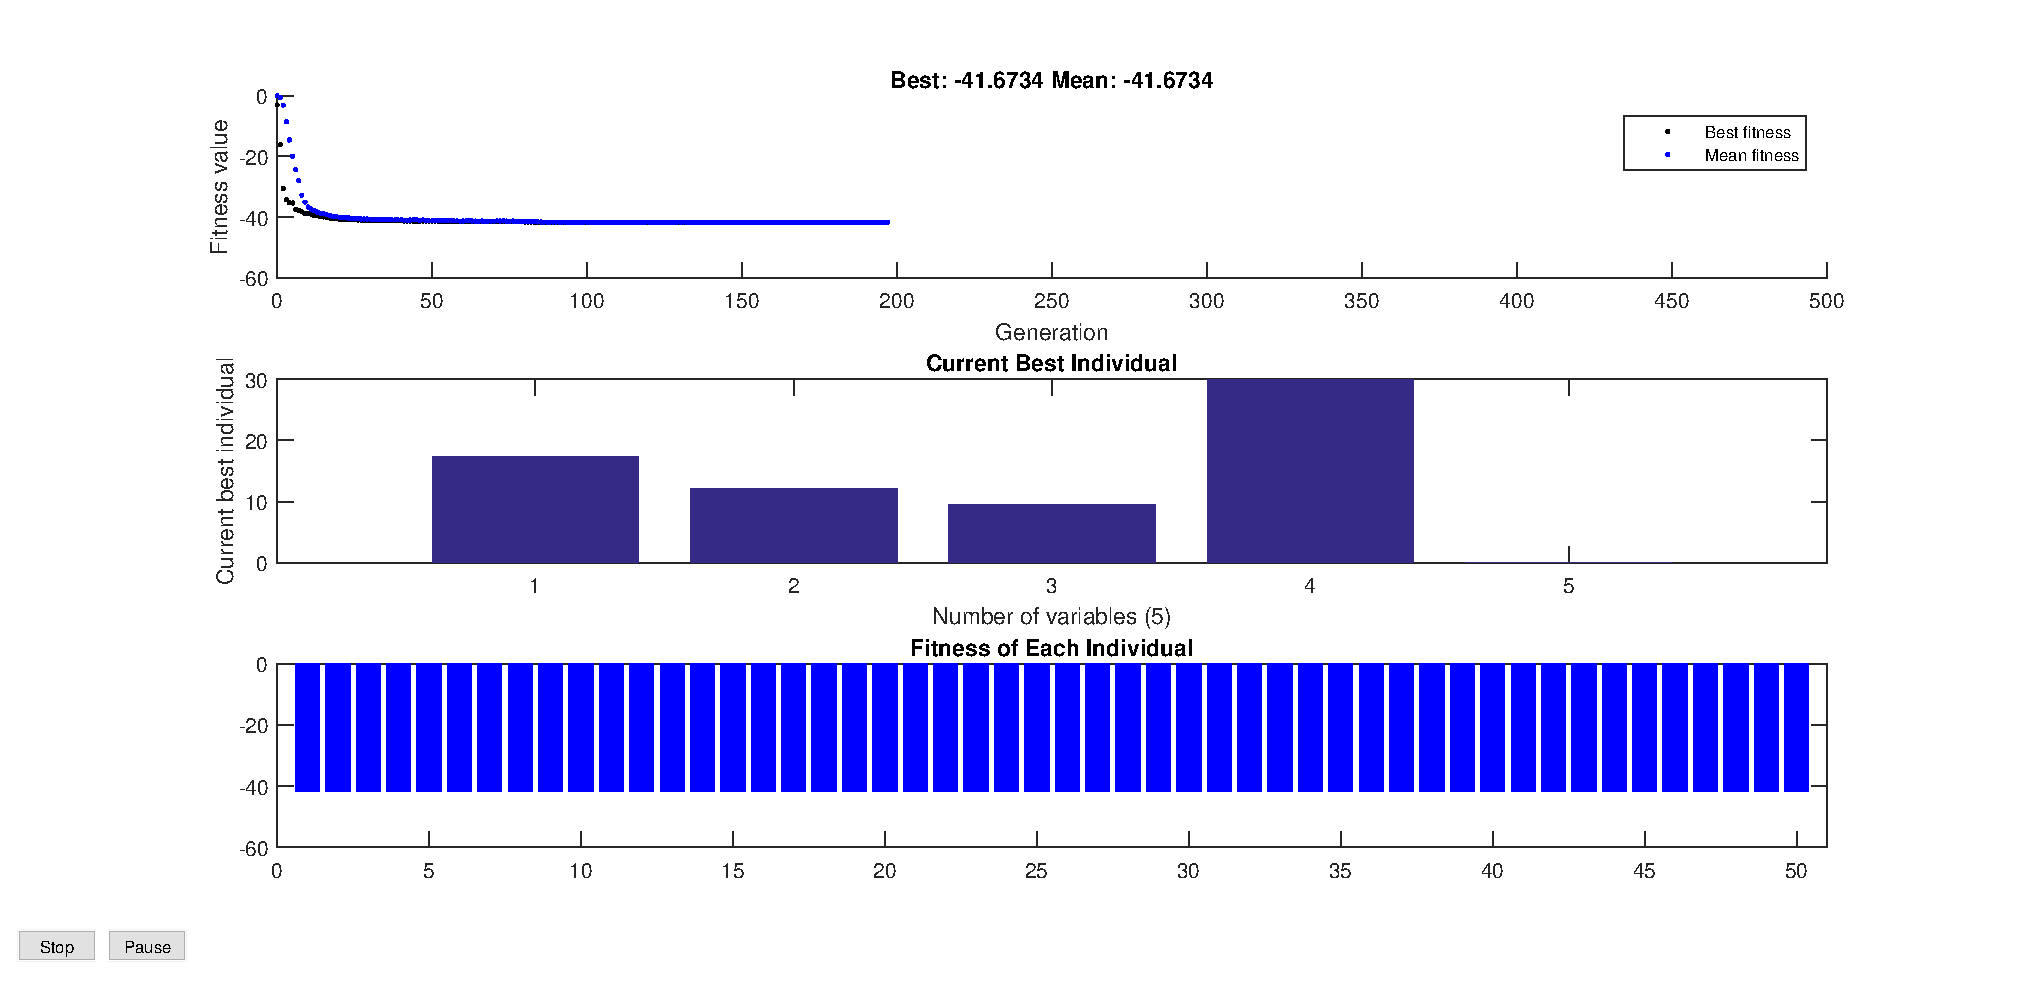
\includegraphics[width=\columnwidth]{1GA.eps}
    \caption{Training process and other element provided by GA method based on short-term harvest}
    \label{fig1}
\end{figure}
\begin{figure}[h]
    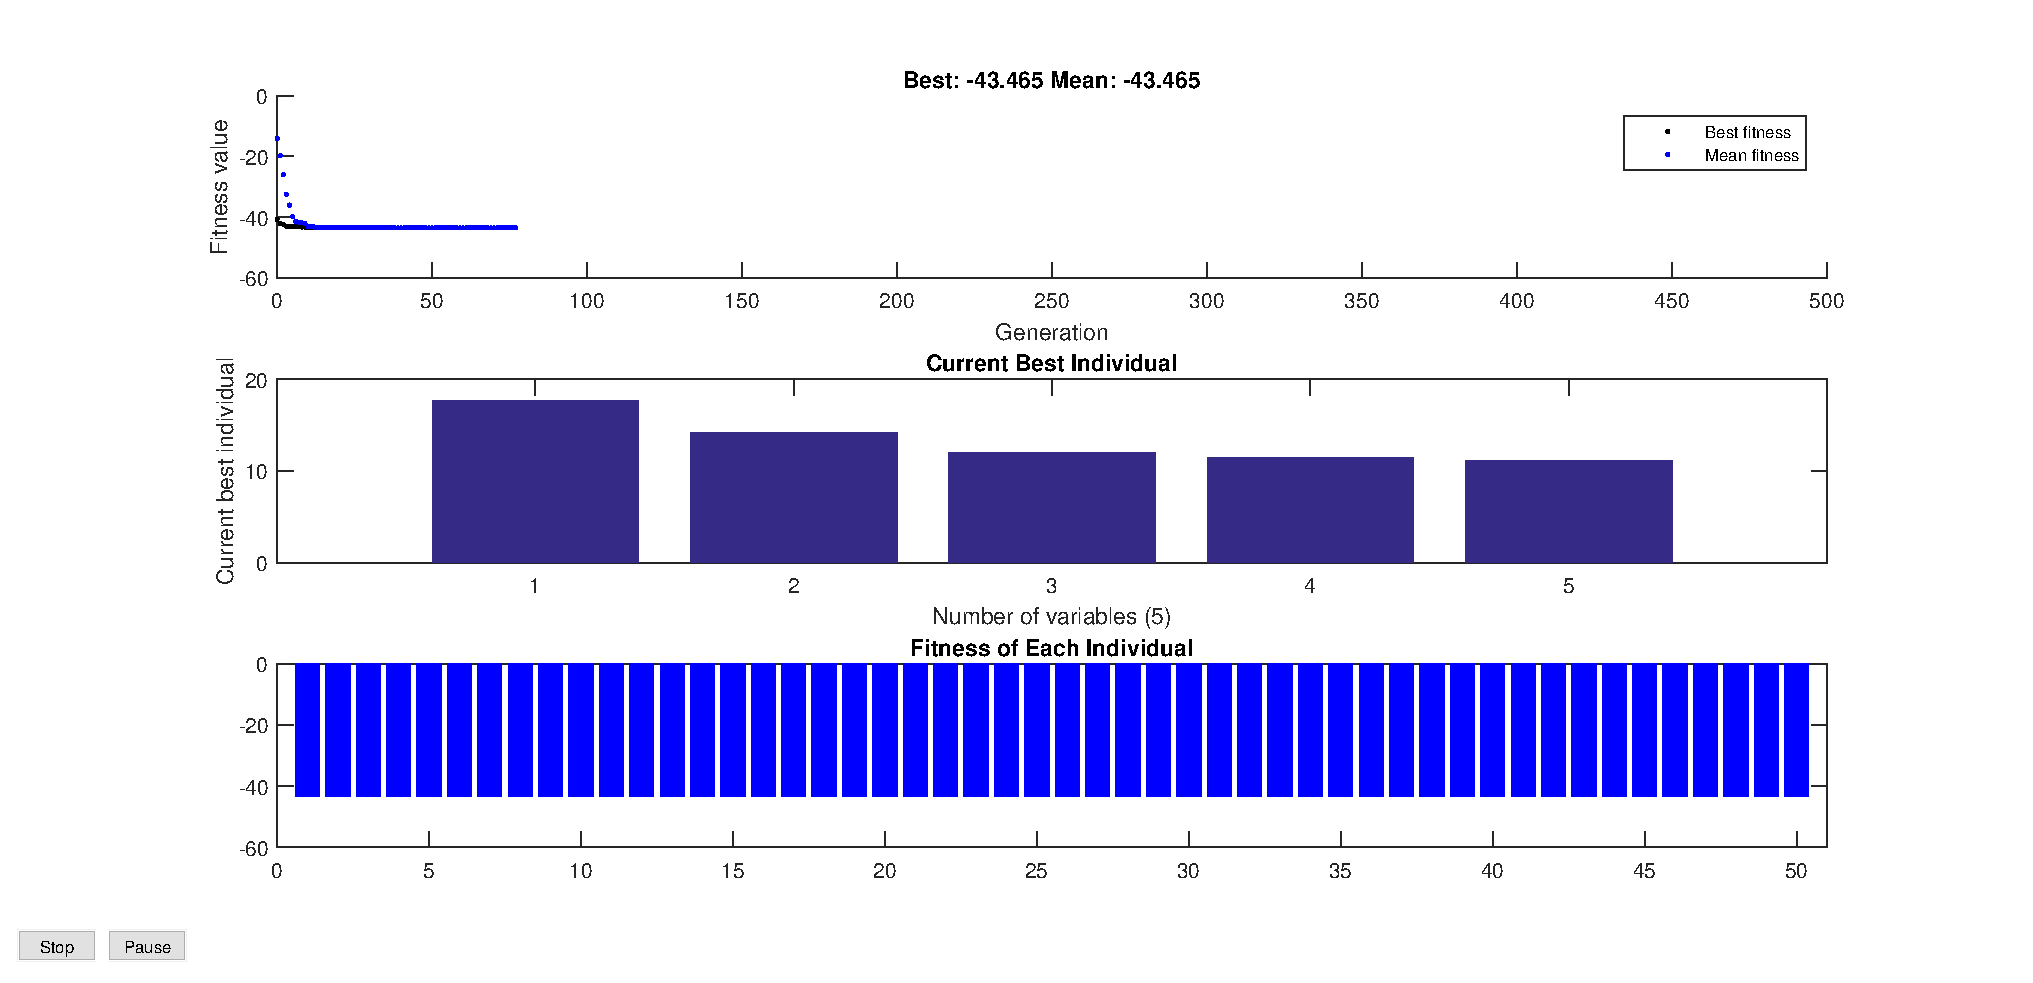
\includegraphics[width=\columnwidth]{2GA.eps}
    \caption{Training process and other element provided by GA method based on long-term harvest}
    \label{fig2}
\end{figure}

\begin{table*}
    \normalsize
    \caption{The fishing strategy and the sum of the harvest}
    \label{tab1}
    \begin{tabular}{ccccccc}\toprule
        Object function and method & $1^{st}$ year & $2^{nd}$ year & $3^{rd}$ year & $4^{th}$ year & $5^{th}$ year & Sum of harvest \\ 
        \midrule
        Gradient Descent & 18.59 & 15.09 & 17.77 & 17.42 & 17.56 & $5.0257\times10^{11}$\\
        Genetic Algorithm with Short-term Assessment & 17.3831 & 12.0797 & 9.4566 & 30.0000 & 0.0001 & $4.2920\times10^{11}$\\ 
        Genetic Algorithm with Long-term Assessment & 17.6717 & 14.1999 & 12.0285 & 11.4857 & 11.1067 & $4.8420\times10^{11}$\\
        \bottomrule
    \end{tabular} 
\end{table*}

\subsection{Solution to the second problem using Harvest Penalty}

In practice, we use genetic algorithm in MATLAB\textsuperscript\textregistered \ toolbox\textsuperscript{\cite{MATLABOptimizationToolbox}} to optimize the object function with Harvest Penalty, i.e. eq. \ref{eq11}, eq. \ref{eq12}, the training process are showned in fig. \ref{fig1} (with short-term harvest penalty) and fig. \ref{fig2} (with long-term harvest penalty). We could find out that if we only take the short-term assessment, the best strategy is fish all of the fish in the 4\textsuperscript{th} year and give up fishing in the 5\textsuperscript{th} year. In this case, the 3-aged fish and 4-aged fish is extinct at the end of 4\textsuperscript{th}, at the beginning of 5\textsuperscript{th} year, the 4-aged fish is still extinct and the 3-aged is revitalized by the 2-aged fish in the 4\textsuperscript{th} year. At the end of 5\textsuperscript{th} year, there are much fewer egg for there are no 4-aged fish. As a result, in the 6\textsuperscript{th} year, the 3-aged fish and the 4-aged fish is just the same with the saturation one, however, the 1-aged fish is extinct (due to the extinction of eggs at the end of 5\textsuperscript{th} year). 

In the above analysis, we can conclude that the short-term assesssment is not conceivable comparing to the long-term one. As for the long-term one, we can find out that the fishing intensity in the 1\textsuperscript{st} year is larger than the other 4 years, which is because the amount of fish in the beginning is a little bit larger than the saturation one, that means even if the fishing intensity is relatively low, the number of fish will surely decrease to the saturation one, or even lower. Thus, the splendid fishing strategy would contain a fierce fishing intensity in the first year, and a relatively average intensity in the following years. 

To sum up, the fishing strategy and the sum of the harvest in 5 years according to the different object function could be summerized in the following tab. \ref{tab1}

Furthermore, the difference between the G.D. method using the penalty of the number of fish and the long-term harvest G.A. method is that the intensity of the first year is even more forcible than the G.A. method, as a trade-off, the intensity of the second year in G.D. method is a little bit lower than the G.A. method. Nevertheless, this two strategies are almost the same in the sum of harvest. 

\section{Conclusion}

From the first case, we can find out that the intensity of fishing and the total of harvest is not monotonous. Which is to say, a larger fishing intensity does not mean a larger harvest. Thus, the concept of scientific development is of exteremely important. In fact, the `fishing intensity'  in the model cannot be directly applied to the actual production activities. The accurate value of this intensity is also useless. In the actual activities, the fishermen should choose a apt intensity, which might be about $k = 15$ in our model to get a profitability and sustainability fishing environment.

From the second case, we can conclude that in a relatively long-term operation of fishing, it is a wise idea to choose a time-varying fishing method. Though according to the different model and different optimizer, the accurate of fishing intensity is different, the total harvest would be about $4.5\sim 5.0 \times 10^{11}\mathrm g (4.8 \times 10^{11} \mathrm g)$ in our model. As mentioned above, the accurate number of intensity is meaningless, however, according to our model, there are two method for the fishermen to choose, which lead to almost the same result in the sum of the harvest.

\begin{itemize}
    \item {Choose a fierce fishing intensity in the first year, and take a short break on the second year, finally, finally, choose a `normal' intensity in the following years}
    \item {Choose a fierce (but moderate than the first one) fishing intensity in the first year, and decrease the intensity year by year at a very low decreasing rate}
\end{itemize}

Though different from each other, these two strategy have something in common:

\begin{itemize}
    \item {Choose a fierce fishing intensity in the first year during to the over-saturation initial state}
    \item {Choose a stable intensity in the last few years to get the stable and near saturation stable state}
\end{itemize}

All in all, we can conclude that the outlook of sustainable development is important and by making the fishing schdeule properly, fishermen tend to get more profit, while the environment is also benefit from this concept.

By a logical extension of this point, we can conclude that the Scientific Outlook of Development will absolutely benefit both the production and environment with the properly modeling and optimizing of the problems in practive. Taking the saying of President Xi as the final conclusion: ``\textbf{\textit{While we want prosperity and wealth, we also want clear waters and green mountains. In fact, clear waters and green mountains can bring us prosperity and wealth.}}''

\section*{Acknowledgement}
\bibliographystyle{ieeetran}
\bibliography{reference}
\end{document}